%! TEX program = xelatex
% \PassOptionsToPackage{draft}{graphicx}
\documentclass{beamer}

\usepackage{kotex}
\usepackage{xcolor}

\usepackage{setspace} % setstretch

\usepackage{tabularray}
\UseTblrLibrary{booktabs}
\UseTblrLibrary{counter}
\usepackage{empheq}
\usepackage[many]{tcolorbox}

%%% Math settings
\usepackage{amssymb,amsmath,mathtools} % Before unicode-math
\usepackage[math-style=TeX,bold-style=TeX]{unicode-math}

%%% Font settings
\setmainfont{Libertinus Serif}
% \setsansfont{Libertinus Sans}[Scale=MatchUppercase]
% \setmonofont{Inconsolata}[Scale=MatchLowercase]
\setmathfont{Libertinus Math} % Before set*hangulfont
\setmathfont{TeX Gyre Pagella Math}[range={\lbrace,\rbrace},Scale=1.1]
\setmainhangulfont{Noto Serif CJK KR}
\setsanshangulfont[BoldFont={* Bold}]{KoPubWorld Dotum.ttf}
% \setmonohangulfont{D2Coding}

%%% PL constructs
\usepackage{ebproof}
\ebproofset{left label template=\textsc{[\inserttext]}}

% For simplebnf
\newfontfamily{\fallbackfont}{EB Garamond}
\DeclareTextFontCommand{\textfallback}{\fallbackfont}
\usepackage{newunicodechar}
\newunicodechar{⩴}{\textfallback{⩴}}

\usepackage{simplebnf}
\RenewDocumentCommand\SimpleBNFDefEq{}{\ensuremath{⩴}}

% because of simplebnf
\newcommand*\vbar{|}
\newcommand*{\finto}{\xrightarrow{\text{\textrm{fin}}}}
\newcommand*{\istype}{\mathrel{⩴}}
\newcommand*{\ortype}{\mathrel{|}}

% for complement
\newcommand{\loverbar}[1]{\mkern 1.5mu\overline{\mkern-1.5mu#1\mkern-1.5mu}\mkern 1.5mu}

\newcommand*{\Reanalyze}{\textit{ReAnalyze}}

% uparrow drawing
\newcommand\xuparrow[1][2ex]{%
   \mathrel{\rotatebox[origin=c]{90}{$\xrightarrow{\rule{#1}{0pt}}$}}
}
\newcommand\xdownarrow[1][2ex]{%
   \mathrel{\rotatebox[origin=c]{90}{$\xleftarrow{\rule{#1}{0pt}}$}}
}

% bra-ket
\newcommand*\bra[1]{\langle{#1}|}
\newcommand*\ket[1]{|{#1}\rangle}

%%%%%%%%%%%%%%%%%%%%%
%  Beamer Settings  %
%%%%%%%%%%%%%%%%%%%%%
\usetheme[numbering=fraction,progressbar=frametitle]{metropolis}
\useoutertheme[subsection=false]{miniframes}
\usecolortheme{rose}

\setbeamertemplate{itemize item}[square]
\setbeamertemplate{itemize subitem}[triangle]
\setbeamertemplate{itemize subsubitem}[circle]

% Custom commands
\usepackage{listings}
\lstdefinestyle{mystyle}{
    basicstyle=\ttfamily\footnotesize
}
\lstset{style=mystyle}

\usepackage{pgfplots}
\usetikzlibrary{shapes,arrows}

\usepackage{adjustbox}
\newcommand{\cfbox}[1]{\adjustbox{cfbox=#1}}

% Define block styles
\tikzstyle{decision} = [diamond, draw, fill=blue!20,
    text width=4.5em, text badly centered, node distance=3cm, inner sep=0pt]
\tikzstyle{block} = [rectangle, draw, fill=white!20,
    text width=10em, text badly centered, rounded corners, minimum height=2em]
\tikzstyle{line} = [draw, -latex']

\title{Squeezed Vacuum States of Light}
\subtitle{Exploring Numerical Simulations Under Multiple Conditions}
\author{이준협, 정윤찬}
\date{SNU Laser Laboratory}
\institute{전기공학설계프로젝트 중간발표\\2023년 3월 23일}

\titlegraphic{%
  \begin{tikzpicture}[overlay,remember picture]
    \node at (current page.145) [xshift=3em, yshift=-1.3em] {
      
\includegraphics[width=3em]{snu-symbol.png}
    };
    \node at (current page.35) [xshift=-3em, yshift=-1.3em] {
      
\includegraphics[width=4em]{laser-symbol.jpg}
    };
  \end{tikzpicture}%
}

\begin{document}
\maketitle

\section{Background}

\begin{frame}[c]
  \frametitle{Introduction: What is Squeezed Light?}
  \[
    \Delta x\Delta p \ge \frac{\hbar}{2}\qquad
    \text{The Uncertainty Principle}
  \]
  \[
    \vec{E}_{\mathbf{k},\lambda}(\vec{r},t)=\vec{e}_{\mathbf{k},\lambda}(p\cos{(\mathbf{k}\cdot\vec{r}-ckt)}+q\sin{(\mathbf{k}\cdot\vec{r}-ckt)})\quad
    \text{TEM field}
  \]
  \[
    \Delta p\Delta q \ge \frac{\hbar ck}{2\varepsilon_{0}L^{3}}\qquad
    \text{Uncertainty Principle for }\vec{E}
  \]
  \pause
  \[
    \text{We want to modulate }\Delta p\text{ and }\Delta q\text{ while preserving the uncertainty}
  \]
\end{frame}

\begin{frame}[c]
  \frametitle{Background: Quantization of the Maxwell Equations}
\[
  \vec{E}=-\nabla\phi-\partial_{t}\vec{A}\qquad
  \vec{B}=\nabla\times\vec{A}\qquad
  \text{The potentials}
\]
\onslide+<2->
\[
  \left(\nabla^{2}-\frac{1}{c^{2}}\partial_{t}^{2}\right)\vec{A}=-\mu_{0}\underbracket{\vec{J}}_{=0}-\nabla(\partial_{t}\phi+\underbracket{\nabla\cdot\vec{A}}_{=0}),\qquad
  \nabla^{2}\phi=-\underbracket{\rho}_{=0}-\partial_{t}(\underbracket{\nabla\cdot\vec{A}}_{=0})
\]
\onslide+<3->
\begin{empheq}[box=\tcbhighmath]{align*}
  \vec{A}=\vec{\alpha}e^{i(\mathbf{k}\cdot\vec{r}-\omega_{\mathbf{k}}t)}\Rightarrow\omega_{\mathbf{k}}^{2}=c^{2}k^{2}\wedge\vec{\alpha}\cdot\mathbf{k}=0\qquad
  \text{Harmonic Oscillator}\\
  \vec{A}_{\mathbf{k},\lambda}=\vec{e}_{\mathbf{k},\lambda}\mathsf{Re}\{\alpha_{\mathbf{k},\lambda}e^{i(\mathbf{k}\cdot\vec{r}-ckt)}\}(\mathbf{k}=2\pi(m,n,l)/L,\lambda=1,2)\quad\text{Per-mode}\\
  \hat{\alpha}_{\mathbf{k},\lambda}=(2\hbar/\varepsilon_{0}L^{3}ck)^{1/2}\hat{a}_{\mathbf{k},\lambda}\qquad
  \text{Annihilation operator for each mode}
\end{empheq}
\end{frame}

\begin{frame}[c]
\frametitle{Background: Squeezing, Wigner Function}
  \[\ket{\psi}\mapsto S(\zeta)\ket{\psi}\qquad
    \text{Unitary transformation}
  \]
  \onslide+<2->
  \[S(\zeta)=\exp(i\cdot\mathsf{Im}\{\zeta^{*} \hat{a}^{2}\})\qquad
    \text{Squeeze by }e^{|\zeta|}\:\text{rotate by}\arg{\zeta}/2
  \]
  \onslide+<3->
  \[
    \text{What do you squeeze? The ``pdf''}
  \]
  \onslide+<4->
  \[
    W(x,p)=\frac{1}{\pi\hbar}\int_{-\infty}^{\infty}\psi^{*}(x+y)\psi(x-y)e^{2ipy/\hbar}dy\qquad
    \text{Wigner function}
  \]
  \[
    \frac{1}{\pi\hbar}\int_{-\infty}^{\infty}e^{-i\alpha(x+y)^{2}}\psi^{*}(x+y)\psi(x-y)e^{i\alpha(x-y)^{2}}e^{2ipy/\hbar}dy=W(x,p-2\hbar\alpha x)
  \]
  \[
    \text{Intuitive calculation: A linear map with determinant 1}
  \]
\end{frame}

\begin{frame}[c]
\frametitle{Background: SHG, Lindblad Equation}
  \[
    \text{Higher-order polarization effect generates multiple frequencies}
  \]
  \[
    \hat{H}=\hbar\omega \hat{b}^{\dag}\hat{b}+\hbar\omega_{P}\hat{a}^{\dag}\hat{a}+i\hbar\chi(\hat{b}^{2}\hat{a}^{\dag}-(\hat{b}^{\dag})^{2}\hat{a})
  \]
  \[
    \text{Second-order interaction: One }\hat{a}\leftrightarrow\text{Two }\hat{b}
  \]
  \[
    \text{Approximate: }\hat{a}\text{ very strong}\Rightarrow\hbar\omega \hat{b}^{\dag}\hat{b}+\mathsf{Im}\{ce^{i\omega_{P}t}\hat{b}^{2}\}
  \]
  \onslide+<2->
  \[
    \text{Interaction with the environment: Lindblad Equation}
  \]
  \[
    \partial_{t}\rho=-\frac{i}{\hbar}[H_{sys},\rho]+\frac{1}{2}\sum_{n}(2C_{n}\rho C_{n}^{\dag}-\rho C_{n}^{\dag}C_{n}-C_{n}^{\dag} C_{n}\rho)
  \]
\end{frame}

\section{Methodology}
\begin{frame}[c]
  \frametitle{Methodology}
  \begin{columns}
    \begin{column}{0.5\textwidth}
      \begin{block}{How to solve}
      \begin{itemize}
        \item Projection onto finite dimemsional Hilbert space spanned by $\{\ket{i}\}_{0\le i\le n}$
        \item Use the open-source Python library QuTiP to solve the Lindblad equation
      \end{itemize}
      \end{block}
    \end{column}
    \pause
    \begin{column}{0.5\textwidth}
      \begin{block}{What to solve}
      \begin{itemize}
        \item No interaction with environment
        \item Interaction with $C=\sqrt{\gamma}\hat{b}$ (Thermal loss)
        \item Higher order generation
      \end{itemize}
      \end{block}
    \end{column}
  \end{columns}
\end{frame}

\section{Results}
\begin{frame}[c]
  \frametitle{Comparison between lossy and non-lossy probabilities}
  \begin{columns}
  \begin{column}{0.5\linewidth}
  \begin{figure}
  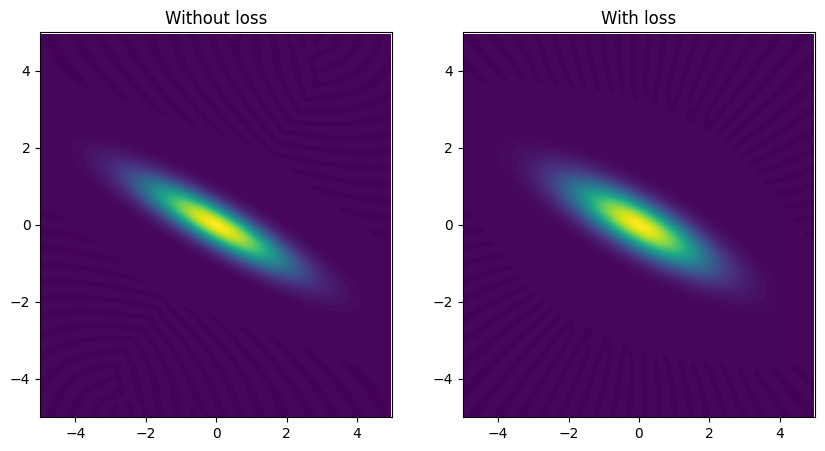
\includegraphics[width=0.7\linewidth]{squeezed_decay_0.2.png}
  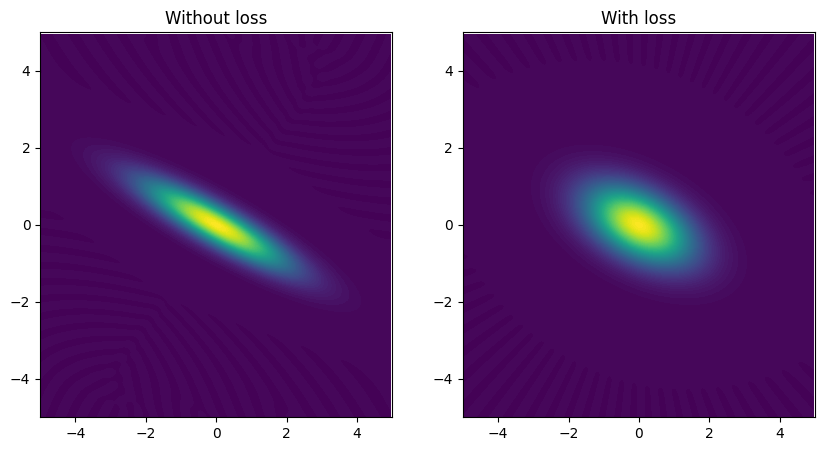
\includegraphics[width=0.7\linewidth]{squeezed_decay_0.5.png}
  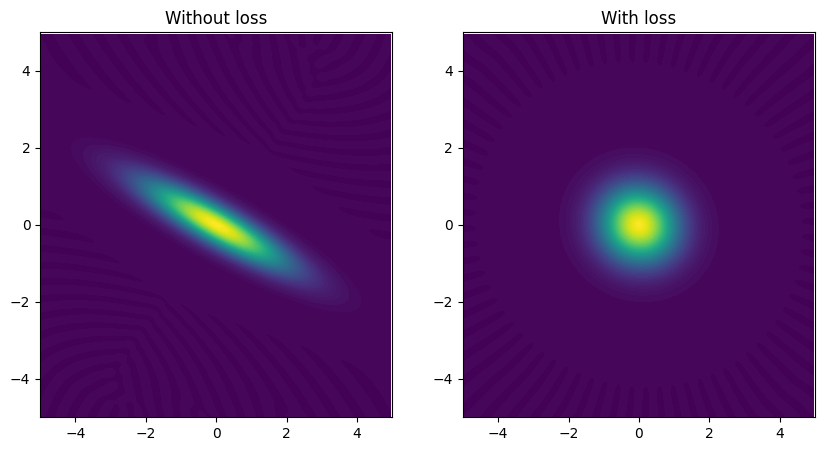
\includegraphics[width=0.7\linewidth]{squeezed_decay_1.0.png}
  \end{figure}
  \end{column}
  \begin{column}{0.5\linewidth}
    \begin{itemize}
      \item Adjust $\sqrt{\gamma}$ in $C=\sqrt{\gamma}\hat{b}$ of the Lindblad equation. $\sqrt{\gamma}=0.2,0.5,1.0$, and the plots are taken after 5 seconds of time evolution.
      \item Since the environment absorbs the photons, the nonlinear effects are diminished.
    \end{itemize}
  \end{column}
  \end{columns}
\end{frame}

\begin{frame}[c]
  \frametitle{Third-order generation?}
  \begin{columns}
    \begin{column}{0.5\linewidth}
    \begin{figure}
    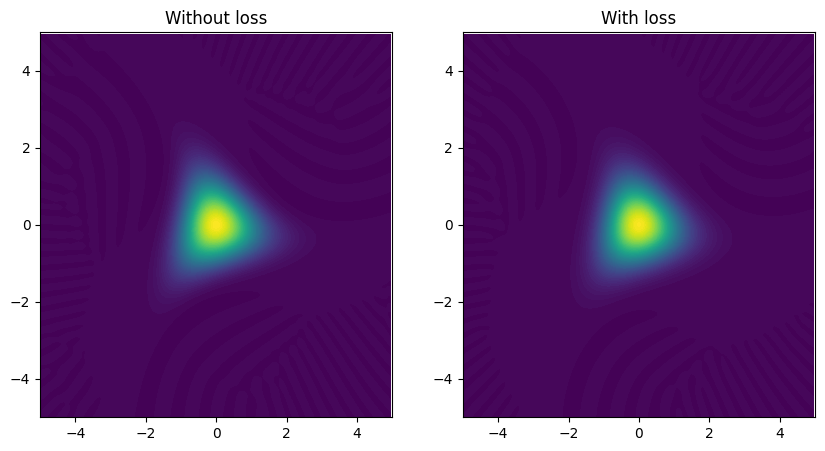
\includegraphics[width=0.7\linewidth]{third_decay_0.2.png}
    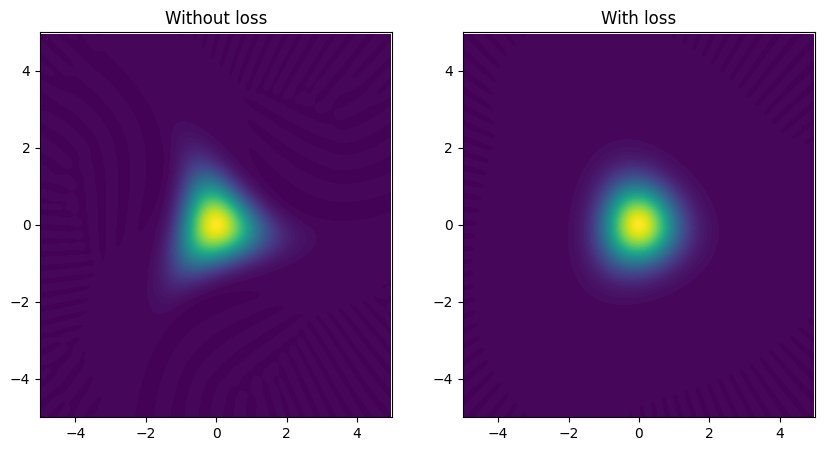
\includegraphics[width=0.7\linewidth]{third_decay_0.5.png}
    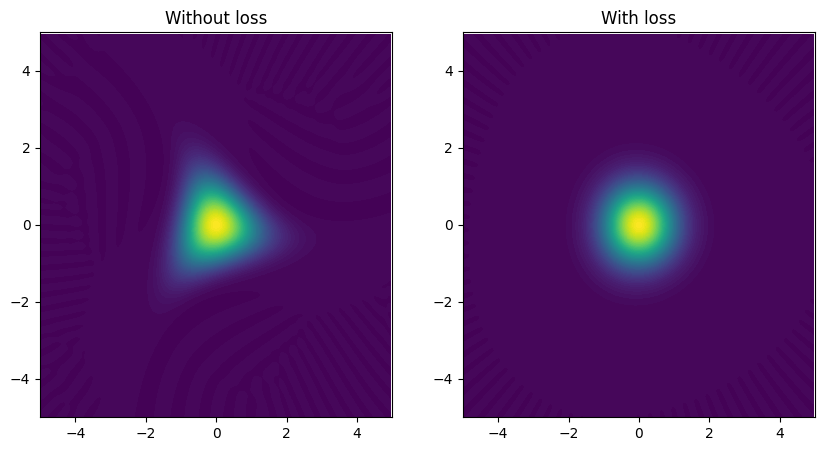
\includegraphics[width=0.7\linewidth]{third_decay_1.0.png}
    \end{figure}
    \end{column}
    \begin{column}{0.5\linewidth}
      \begin{itemize}
        \item The same plots, with $H_{sys}$ containing $\hat{b}^{3}$
        \item Expected the Wigner function to turn into transform into the form $W(2^{nd},2^{nd})$
      \end{itemize}
    \end{column}
  \end{columns}
\end{frame}

\begin{frame}[c]
  \frametitle{Summary}
  \begin{itemize}
     \item Studied: what are squeezed states, how to generate them
     \item Tried out: the QuTiP library to simulate interaction with the environment and higher order generation
  \end{itemize}
\end{frame}

\begin{frame}[c]
\frametitle{References}
\footnotesize{
\begin{thebibliography}{99} % Beamer does not support BibTeX so references must be nserted manually as below
\bibitem[Loudon]{p1} R. Loudon, \textit{The Quantum Theory of Light.} Oxford, UK: OUP Oxford, 2000.
\bibitem[Lindblad]{p2} H. Seifoory, S. Doutre, and M. M. Dignam, ``The properties of squeezed optical states created in lossy cavities,'' 2016. [Online]. Available: arXiv:1608.05005[quant-ph].
\bibitem[QuTiP]{p3} J. R. Johanssona, P. D. Nationa, F. Nori, ``QuTiP: An open-source Python framework for the dynamics of open quantum
systems,'' 2011. [Online]. Available: arXiv:1110.0573[quant-ph].
\end{thebibliography}
}
\end{frame}

\begin{frame}[c]
  \centering\LARGE
  감사합니다\\[\baselineskip]
\end{frame}
\end{document}
%%% Local Variables:
%%% coding: utf-8
%%% mode: latex
%%% TeX-engine: xetex
%%% End:
